% !TEX root = /home/fred-olav/afgv/src/preamble.tex
%(BEGIN_QUESTION)


Use Bernoulli's equation to calculate the hydrostatic pressure at the bottom of this water storage tank:

$$\includegraphics[width=9cm]{i02987x01.eps}$$

\noindent
{\bf Bernoulli's equation:}

$$z_1 \rho g + {v_1^2 \rho \over 2} + P_1 = z_2 \rho g + {v_2^2 \rho \over 2} + P_2$$

\vskip 10pt

\noindent
Where,

$\rho$ = 1000kg/m$^{3}$ (for vann)

$g$ = 9.81 m/s$^{2}$

\vskip 10pt

\underbar{file i02987}
%(END_QUESTION)





%(BEGIN_ANSWER)

$P$ = 68670Pa = 0.6867 Bar

%(END_ANSWER)





%(BEGIN_NOTES)

%INDEX% Physics, static fluids: Bernoulli's equation applied to hydrostatic head
%INDEX% Physics, static fluids: hydrostatic pressure

%(END_NOTES)


